\chapter{Vista l\'ogica}
\section{Introducci\'on}
Muestra los componentes principales del dise\~no del sistema y sus relaciones, de forma independiente de los detalles técnicos y de c\'omo la funcionalidad debe ser implementada. 

\section{Visión general}
El sistema EHC está descompuesto como se muestra en el diagrama de clase ~\ref{fig:diagramaClase}. En este diagrama, se muestran las principales clases que forman el core de la aplicación y la conexión ente ellas. Cada una de ellas, están representadas por algunas de las funciones y variables más representativas.

\begin{figure}
	\centering
	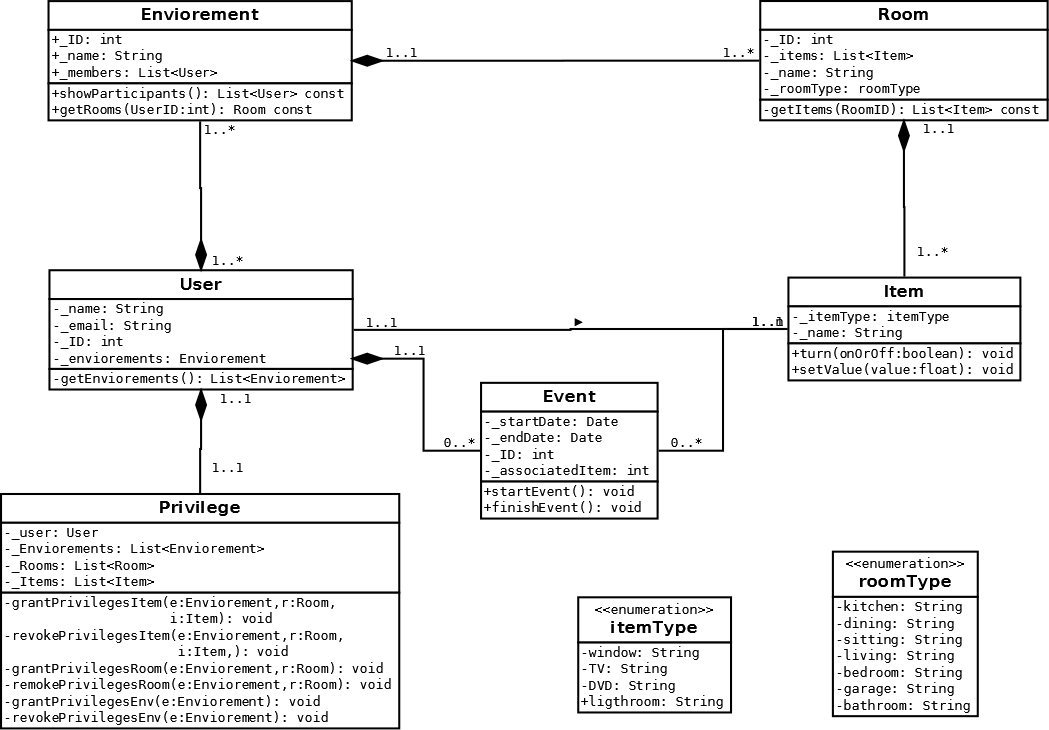
\includegraphics[width=0.8\textwidth]{4.Disenio/Imagenes/diagramaClase}
	\caption{Diagrama de clase.}
	\label{fig:diagramaClase}
\end{figure}

Para facilitar la comprensión del sistema, facilitamos el diagrama de secuencia en la figura ~\ref{fig:diagramaSecuencia}. Este diagrama contiene la identificación del usuario en el sistema y a continuación, la petición de control de un dispositivo. 

\begin{figure}[h!]
	\centering
	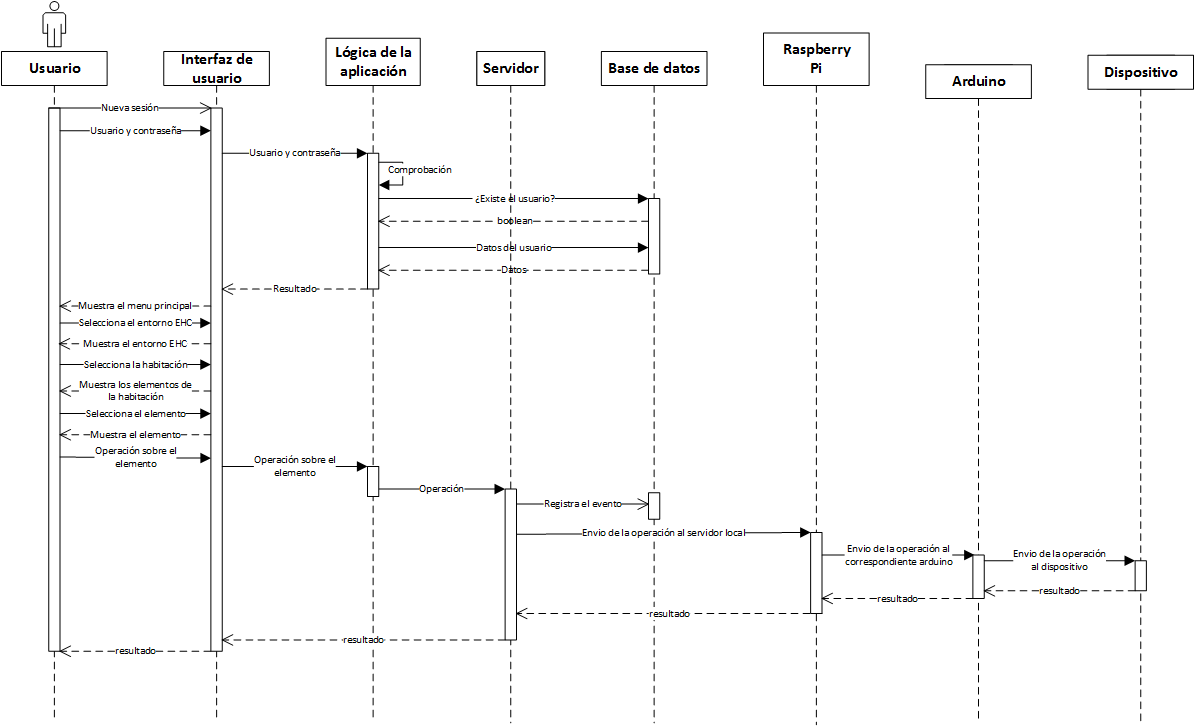
\includegraphics[width=0.9\textwidth]{4.Disenio/Imagenes/DisenioEHC}
	\caption{Diagrama de secuencia de la autentificaci\'on en el sistema y controlar un dispositivo.}
	\label{fig:diagramaSecuencia}
\end{figure}


